% vim: set expandtab sw=2 ts=2 sts=2:
% vim: set spell spelllang=en:

\documentclass{article}

\usepackage[a4paper, total={18cm, 23cm}]{geometry}
\usepackage{polyglossia}
\usepackage{csquotes}
\usepackage{xevlna}
\usepackage{graphicx}

\setmainlanguage{english}

\title{WinMMB crash course}
\date{}

\begin{document}
\maketitle

\noindent The WinMMB is a very thin and dumb GUI to control MMB. WinMMB can start MMB with the given command file and monitor its progress.

\begin{center}
  \noindent Example of WinMMB window with a running simulation: \\
  \vspace{0.5\baselineskip}
  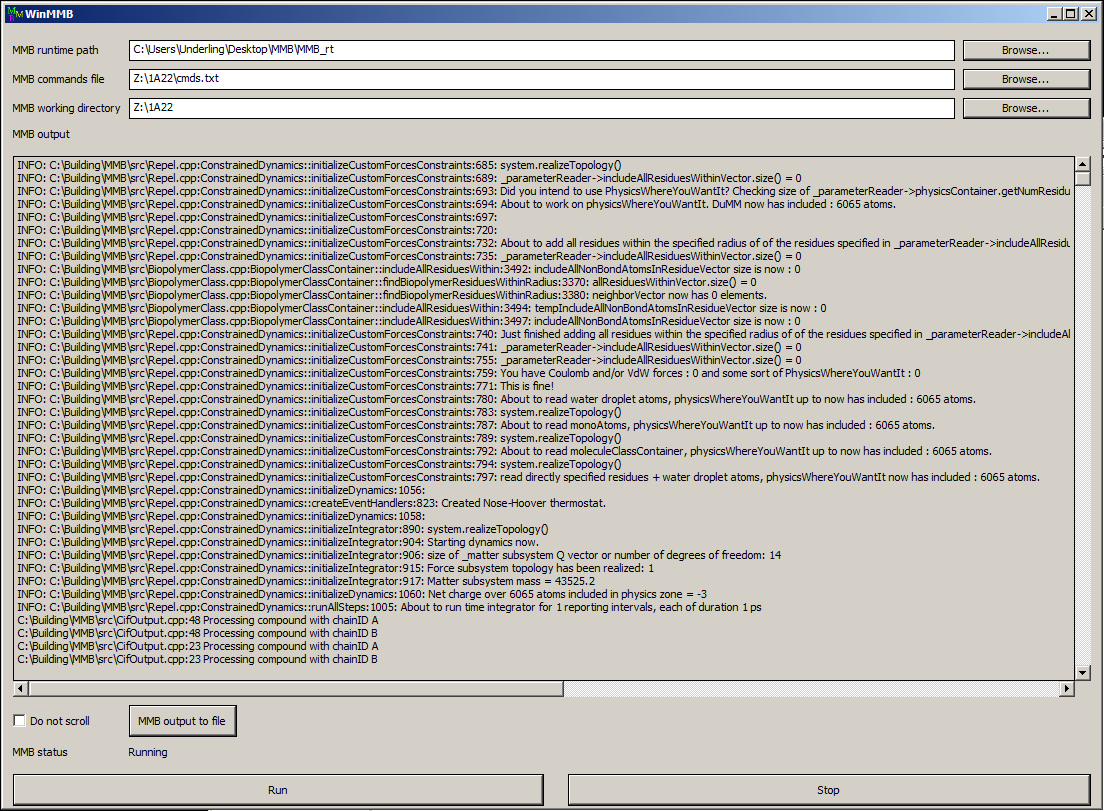
\includegraphics[scale=0.4]{WinMMB.png}
\end{center}

\begin{center}
  \begin{tabular}{lp{7cm}}
    \multicolumn{2}{c}{\enquote{Configuration} options:} \\
    \textbf{MMB runtime path} & Path to a directory with the actual MMB installation. There is no reason to change this value. \\
    \textbf{MMB commands file} & Path to MMB commands file. Set this to point to the commands file of the simulation you want to run. \\
    \textbf{MMB working directory} & MMB will use this directory to write all output of the simulation, e.g. the \emph{trajectory} files. If your simulation reads some input files such as structures, they also need to be placed in this directory.
  \end{tabular}
\end{center}

\begin{itemize}
  \item You can save the MMB progress output to file by clicking on \emph{MMB output to file}
  \item If you leave \emph{MMB working directory} empty, MMB will write the output files to the directory specified by \emph{runtime path}. You most likely do not want this to happen.
  \item You can tell that MMB failed to complete the simulation successfully when \emph{MMB status} reads \emph{Failed}.
\end{itemize}

That's about it\ldots{} have fun!

\end{document}
